\documentclass[10pt]{article}
% Approximates the NeurIPS single-column format: 5.5in x 9in text block, 10pt.
% Substitute the official neurips_20XX.sty before submission; the content and
% structure here are built to that template's requirements (9-page main body,
% unlimited references and appendix, anonymous submission, paper checklist).
\usepackage[textwidth=5.5in,textheight=9in,centering]{geometry}
\usepackage{times}
\usepackage{amsmath,amssymb}
\usepackage{graphicx}
\usepackage{booktabs}
\usepackage{caption}
\usepackage[colorlinks=true,linkcolor=black,citecolor=black,urlcolor=blue]{hyperref}
\usepackage{titlesec}
\usepackage{xcolor}
\usepackage{microtype}

\captionsetup{font=small,labelfont=bf,skip=6pt}
\titleformat{\section}{\large\bfseries}{\thesection}{0.6em}{}
\titlespacing*{\section}{0pt}{10pt}{5pt}
\titleformat{\subsection}{\normalsize\bfseries}{\thesubsection}{0.6em}{}
\titlespacing*{\subsection}{0pt}{8pt}{4pt}

\newcommand{\keyfinding}[1]{\vspace{2pt}\noindent\fbox{\parbox{0.97\linewidth}{\small #1}}\vspace{2pt}}

\title{\bf A Memory That Only Looks Like One:\\[2pt]
\large The Recurrent State of a Hybrid Vision-Language Model Relays\\
the Picture Rather Than Storing It}

\author{Raj Dandekar \quad Rajat Dandekar \quad Sreedath Panat\\[3pt]
Vizuara AI Labs\\
\texttt{research@vizuara.com}}
\date{}

\begin{document}
\maketitle

\begin{abstract}
\noindent
A hybrid vision-language model carries two kinds of memory. Its attention
layers keep a growing cache: every token the model reads, including every patch
of an image, is stored as a key-value entry that later tokens can look up. Its
recurrent layers keep a single state of fixed size, and every new token
overwrites part of that state. Prior work proved that a fixed-size state must
eventually lose information. It does not tell us \emph{when} a given model
forgets, \emph{what} it keeps while forgetting, or \emph{what breaks}
downstream. We answer these three questions for Zamba2-VL-7B, a model in which
all 81 decoder layers carry a Mamba2 recurrent mixer and only 13 also carry
attention.

First, just after reading an image the recurrent state holds the gist, not the
details. A linear probe reads \emph{which} object was in the picture at
$92.5\%$ from the best single layer, against a $12.5\%$ chance rate. The same
probe can barely read \emph{how many} objects there were or \emph{where} they
sat.

Second, how fast that memory fades can be computed from the weights alone.
Mamba2 multiplies its state by $\exp(\Delta_t A)$ at every token, so retention
after $k$ tokens is $\exp(A\sum\Delta_t)$, and each head has a half-life of
$\ln 2/(|A|\bar{\Delta})$ tokens. The median predicted half-life is $6.6$
tokens in the 7B model, and $2.9$ and $2.6$ in its two smaller siblings, with
nothing fitted.

Third, and this is the central result: the memory a probe appears to find at
longer distances is mostly not memory. Splitting heads by predicted half-life
confounds decay with write amplitude, because the same gate sets both, so we
hold the gate fixed and split by the decay weight $|A|$ alone. The ordering
then comes out exactly as decay predicts, but the amounts are impossible.
Heads with a $2.3$-token half-life, whose own parameters keep
$4\times10^{-9}$ of any trace after sixty-four tokens, still decode the object
at $26.6\%$ there. Something must be re-supplying them. Deleting the image's
key-value entries from all 13 attention layers immediately after the image,
without touching any recurrent state, collapses the apparent memory: the fast
third of heads falls from $51.6\%$ to $7.8\%$ at thirty-two tokens, below
chance, and at matched write amplitude the deletion costs fast heads $2.4$
times more than slow heads beside the image. The recurrent channel is passing
along what attention still holds; it is not storing the picture.

A direct causal test agrees. Exchanging all 81 recurrent states between two
runs that saw different images changes nothing: $100$ of $100$ answers still
follow the run's own image, with every swap verified. Exchanging seven of the
thirteen attention caches flips $94$ of $100$ answers to the other image.
Finally, the practical consequence for cache pruning: the redundancy premise
behind visual token and key-value pruning survives on this architecture down
to a quarter of the entries, but the cost of pruning harder roughly doubles
with distance. Removing every visual entry costs $34$ accuracy points beside
the image and $59$ at thirty-two tokens.
\end{abstract}

\begin{figure}[t]
\centering
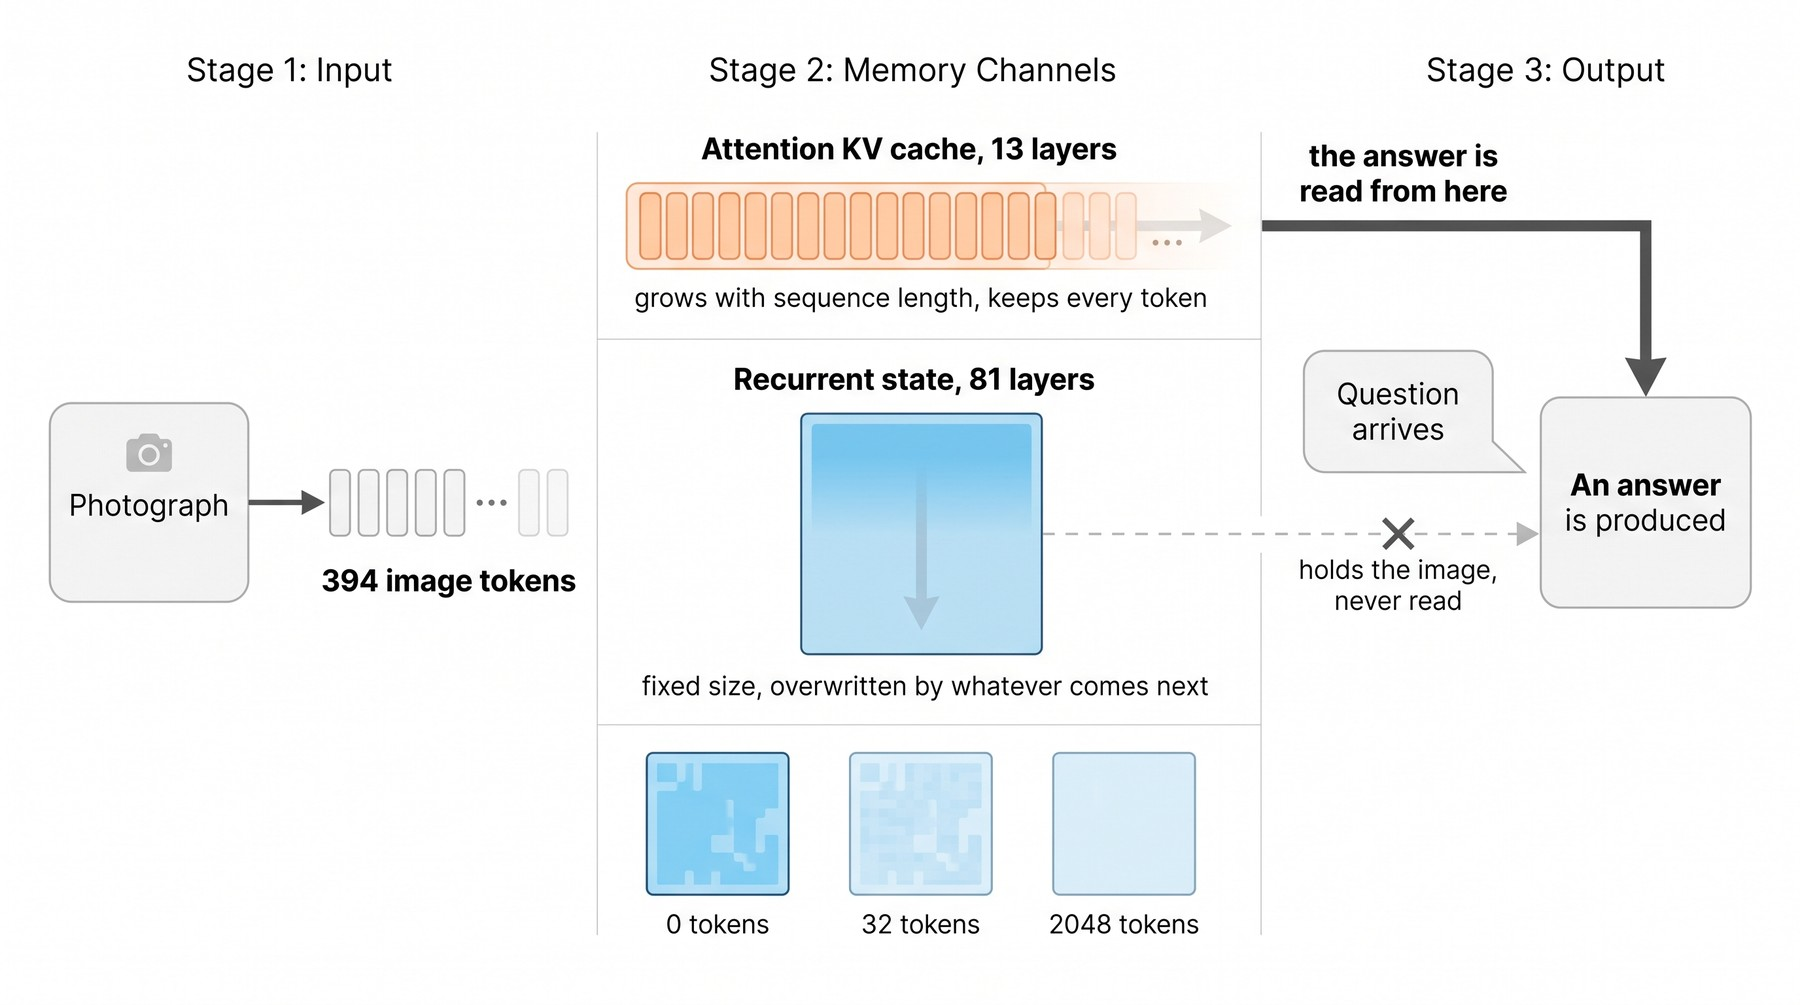
\includegraphics[width=0.94\linewidth]{assets/fig_idea.jpg}
\caption{The two memory channels of a hybrid vision-language model and the
question this paper asks of them.}
\end{figure}

\section{What Was Known Before, and What Is New Here}

Linear-attention and state-space models replace the growing key-value cache of
a transformer with a state of fixed size
\cite{katharopoulos2020linear,gu2022s4,peng2023rwkv,gu2023mamba,dao2024mamba2,beck2024xlstm}.
A fixed state cannot grow with the context. For this reason, most deployed
systems keep a few attention layers alongside the recurrent ones, and these
hybrid models are now common
\cite{lieber2024jamba,glorioso2024zamba,de2024griffin,ren2025samba,waleffe2024empirical}.
This paper asks a simple question about such a model: what is the recurrent
half actually holding?

We want to be clear about what is already known. Prior work established that a
fixed-size recurrent state must eventually lose information from context; that
premise is not ours. Jelassi et al.\ \cite{jelassi2024copying} prove that
transformers can copy exponentially long strings while state-space models are,
in their words, ``fundamentally limited by their fixed-size latent state''.
They also show empirically that pretrained transformers ``dramatically
outperform state space models at copying and retrieving information from
context''. Other results reach the same conclusion from other directions.
State-space models are limited to $\mathrm{TC}^0$ and cannot reliably track
state \cite{merrill2024illusion}. In-context retrieval is the specific skill
that separates recurrent models from transformers \cite{wen2024rnns}. Most of
the quality gap between efficient architectures and attention comes from recall
\cite{arora2023zoology,arora2024based}. Our work builds on these results; it
does not rediscover them.

Table~\ref{tab:novelty} states what that literature establishes and what this
paper adds.

\begin{table}[h]
\centering\small
\begin{tabular}{p{0.44\linewidth}p{0.48\linewidth}}
\toprule
\textbf{Established by prior work} & \textbf{New here} \\
\midrule
A fixed-size state must lose information from context, with a capacity proof
and behavioural evidence \cite{jelassi2024copying,merrill2024illusion,wen2024rnns}.
& \emph{When}. A retention horizon in tokens, computed from the model's own
$A$ and $\Delta$ with nothing fitted, at three scales. \\
\addlinespace
Recurrent models underperform at copying and retrieval as a class
\cite{arora2023zoology,arora2024based}.
& \emph{What survives}. The failure is content-selective: object identity is
highly decodable at the same instant that count and position are near chance. \\
\addlinespace
Architectures are compared to one another from the outside.
& \emph{Causal localisation inside one model}, and the finding that the
recurrent channel relays rather than stores, which makes probing it at distance
a measurement of the attention channel. \\
\addlinespace
Visual tokens and key-value entries carry substantial redundancy that can be
pruned \cite{chen2024fastv,yang2024visionzip,shang2025prumerge}.
& \emph{What underwrites that premise}, and that its safety margin shrinks
with distance from the image on a hybrid. \\
\bottomrule
\end{tabular}
\caption{Delineation of prior work and contribution.}
\label{tab:novelty}
\end{table}

\section{Significance}

Why does this matter? Hybrid models are being adopted because a fixed-size
state promises constant-memory inference. Anyone building or deploying one
must then decide how much to trust the recurrent channel: can it be relied on
to carry information across a long prompt? Today that is a judgement call.
This paper turns it into a calculation. Given a checkpoint's decay weight $A$
and its gate statistics, you can compute how many tokens the recurrent state
retains what it wrote, before running any experiment. For Zamba2-VL-7B the
answer is single digits. That is far shorter than one would guess from the
size of the state, which is $458{,}752$ numbers per layer.

There is also a concrete consequence for a popular optimization. A large body
of work speeds up vision-language models by discarding visual tokens or
evicting their key-value entries, on the stated premise that those entries are
largely redundant \cite{chen2024fastv,yang2024visionzip,shang2025prumerge}; a
parallel line evicts key-value entries in language models on similar grounds
\cite{zhang2023h2o,li2024snapkv,xiao2024streaming}. These methods were
developed and validated on dense transformers, where they work. We find that
they mostly survive the move to this hybrid: a quarter of the visual entries
is enough to hold accuracy at both distances we tested. What does not survive
is the safety margin. The redundancy exists because the recurrent channel is
relaying the picture, and it only relays for a few tokens. As a result, the
cost of aggressive pruning roughly doubles between a prompt that asks about
the image immediately and one that asks thirty-two tokens later. A pruning
method tuned on short prompts will therefore look safer than it is. That is
the kind of failure a standard benchmark is least likely to catch.

\section{Model and Instruments}

\subsection{The model}

Zamba2-VL-7B \cite{zamba2vl} is the vision-language member of the Zamba family
\cite{glorioso2024zamba}, which pairs a Mamba2 backbone \cite{dao2024mamba2}
with a shared attention module, and it takes its vision encoder from Qwen2.5-VL
\cite{bai2025qwen25vl}. It is Apache-2.0 licensed and has 81 decoder layers. Every one carries a Mamba2
mixer, and 13 of them additionally carry a shared attention block, at layer
indices 6, 11, 17, 23, 29, 35, 41, 47, 53, 59, 65, 71 and 77. The recurrent
channel therefore spans all 81 layers and the attention channel spans 13. Each
layer's recurrent state is a tensor of shape $[112, 64, 64]$, which is
$458{,}752$ numbers. One image occupies between 345 and 415 tokens depending on
its aspect ratio.

\subsection{Reading the state}

The Mamba2 recurrence is
\begin{equation}
S_t = S_{t-1}\exp(\Delta_t A) + \Delta_t\, x_t B_t^{\top},
\qquad y_t = S_t C_t ,
\end{equation}
so writing uses $(x, B)$, reading uses $C$, and retention of anything already
present is governed by $A$ and $\Delta$ alone. In words: at each token the
state is first multiplied by $\exp(\Delta_t A)$, a number strictly between
zero and one, which shrinks everything the state already holds. Then
$\Delta_t x_t B_t^{\top}$ is added, which is the only operation that writes.
The shrink factor is set by one stored weight $A$ and one input-dependent gate
$\Delta_t$, so each head is a leaky accumulator whose leak rate can be read
off the checkpoint. We verified each of these facts against the installed
model source rather than assuming the canonical form. In particular
$A = -\exp(A_{\log})$ is a per-head scalar, the gate is
$\Delta = \mathrm{softplus}(\Delta_{\text{raw}} + b)$ clamped below at
$0.001$ with no upper clamp, and the decay factor is
$\exp(\Delta_t A)$ elementwise.

To measure what the state holds, we use a linear probe, the simplest possible
reader: a classifier that computes a weighted sum of the state's numbers and
predicts the trial's answer from that sum alone, trained on some trials and
tested on held-out ones. If even this simple reader recovers the answer, the
answer is present in an easily readable form. Probing this way is standard
\cite{alain2016probes}, and its hazards are well known. A probe can
succeed because the classifier is powerful, not because the model uses the
information. This is why probing papers check selectivity against control
tasks \cite{hewitt2019control} and read their results with care
\cite{belinkov2022probing}. We therefore never rely on a probe alone. Every
probe result is paired with an intervention on the model, in the tradition of
causal mediation analysis \cite{vig2020causal} and activation patching
\cite{meng2022rome,wang2022ioi,zhang2024patching}, and we report what each
intervention does to the model's own behaviour, not only to the probe's
readout \cite{zhang2024patching}.

One practical detail: $458{,}752$ numbers per layer is too wide to probe
directly, so each layer's state is first passed through a fixed Gaussian
random projection down to 512 features. By the Johnson-Lindenstrauss property,
such a projection preserves linear separability up to a controlled distortion,
so a linear probe on the projected features is, to that tolerance, a linear
probe on the state itself. The projection columns are drawn independently, so
the first $k$ columns are themselves a valid $k$-feature projection.

\subsection{Splicing the channels}

The splice runs the model twice, on two different images, and then exchanges
one memory channel between the runs while leaving the other untouched. The run
that keeps its own question is called the host; the run that donates its
memory is called the donor. After the exchange, the host answers its question,
and we record whose image the answer describes. Swapping the recurrent channel
replaces all 81 states and convolution buffers; swapping the attention channel
replaces the 13 key and value caches. The host's cache is restored exactly
afterwards, so one prefill supports many conditions.

\section{Materials}

Trials are built from COCO val2017 instance annotations \cite{lin2014coco},
the corpus underlying most visual instruction tuning \cite{liu2023llava}.
There are three question families: which object is present, how many of a
named object are present, and where in the picture a named object is. Every
question is eight-way forced choice, so the chance rate is exactly $12.5\%$.
Trials are constructed in blocks of eight. All eight trials in a block share
one identical candidate list, and each candidate is the correct answer exactly
once within the block. This construction is what makes the pre-image control
meaningful. Because the candidate set is fixed and each answer appears equally
often, a classifier that has not seen the image has nothing to exploit: no
candidate is more likely than any other, so it cannot beat chance.

Images are fetched at native geometry for the decay experiments. For the
splice they are letterboxed onto a common square canvas. The reason is
practical: two runs on images of different shape emit different numbers of
vision tokens, and attention caches of different length cannot be exchanged.
Letterboxing rather than square resizing matters. In a pilot, a plain square
resize deformed the content badly enough to drop identity accuracy from 17 of
30 to 8 of 30.

\section{Result 1: The State Records Gist, Not Particulars}

We first probe the state at distance zero, the instant the image has just been
read. The state is highly informative about which object is present, and close
to uninformative about how many objects or where they are. Probing the full
state across all 81 layers reads identity at $83.1\%$ against a $12.5\%$
chance rate ($p = 6 \times 10^{-92}$, $n = 160$), count at only $19.4\%$
($p = 0.009$), and position at only $17.5\%$ ($p = 0.041$).

In fact these figures understate what the state carries. The full-state
feature vector has $81 \times 512 = 41{,}472$ dimensions, far more than the
number of trials, so the full-state probe overfits, and a probe on a single
layer does substantially better. Layer 64 alone reads identity at $92.5\%$.
The late third of the stack (layers 60 to 81) averages $85.2\%$, against
$56.0\%$ for the middle third. On the identical trials the full-state probe
reads $71.7\%$. Two conclusions follow. The gist is stronger than the
aggregate number suggests, and it is concentrated in the late layers.

\begin{figure}[h]
\centering

\includegraphics[width=\linewidth]{assets/f1_horizon_depth.png}
\caption{\textbf{Left:} identity decoded from the recurrent state against
distance from the image, at three model scales, 120 trials per point. The
pre-image control reads exactly $12.5\%$ at every scale. \textbf{Right:}
identity decoded from each layer's state alone at the instant of writing, with
red marking the 13 layers that also carry attention. A probe given all 81 layers
at once does worse than the best single layer, because $41{,}472$ features on
120 trials is heavily overparameterised.}
\label{fig:horizon}
\end{figure}

\keyfinding{The recurrent state is not a compressed copy of the image. It is a
selective summary that keeps object identity and discards count and position, and
that selection is visible at the instant of writing rather than emerging over
distance.}

\section{Result 2: The Forgetting Horizon, Predicted From the Weights}

\subsection{The prediction}

Retention of whatever the state held, after $k$ further tokens, is
\begin{equation}
R(k) = \exp\!\Big(A \sum_{t=1}^{k}\Delta_t\Big),
\qquad
\text{half-life} = \frac{\ln 2}{|A|\,\bar{\Delta}} .
\end{equation}
$A$ is a stored weight. $\bar{\Delta}$ is measured from the gate channels of the
input projection over the tokens that follow the image, on the same prompts the
decay experiment uses. Nothing here is fitted to a decay curve.

Across all $81 \times 112 = 9{,}072$ heads the predicted median half-life is
$6.6$ tokens, with an interquartile range of $2.8$ to $17.8$. $85.0\%$ of heads
fall below 32 tokens and $0.08\%$ above 512. Measured over eight different
photographs the median moves only between $6.44$ and $6.86$ tokens, so the
horizon is a property of the model rather than of the stimulus.

\subsection{The measurement}

Does the measured decay match this prediction? Our original collection
measured only distances $0$ and $32$, and $32$ tokens is already far past the
region where the prediction changes quickly. Table~\ref{tab:fine} therefore
shows a finer sweep, on 120 identity trials at each of eleven distances.

\begin{table}[h]
\centering\small
\begin{tabular}{rrrrr}
\toprule
tokens & probe accuracy & $p$ & behaviour & predicted retention (median) \\
\midrule
0  & $71.7\%$ & $2\times10^{-50}$ & $94.2\%$ & $1.000$ \\
1  & $60.0\%$ & $2\times10^{-34}$ & $96.7\%$ & $0.901$ \\
2  & $59.2\%$ & $2\times10^{-33}$ & $97.5\%$ & $0.812$ \\
4  & $41.7\%$ & $1\times10^{-15}$ & $96.7\%$ & $0.659$ \\
8  & $35.0\%$ & $2\times10^{-10}$ & $97.5\%$ & $0.434$ \\
12 & $30.0\%$ & $3\times10^{-7}$  & $96.7\%$ & $0.286$ \\
16 & $24.2\%$ & $3\times10^{-4}$  & $97.5\%$ & $0.188$ \\
24 & $29.2\%$ & $1\times10^{-6}$  & $95.8\%$ & $0.082$ \\
32 & $20.8\%$ & $7\times10^{-3}$  & $95.0\%$ & $0.036$ \\
48 & $25.8\%$ & $6\times10^{-5}$  & $97.5\%$ & $0.007$ \\
64 & $21.7\%$ & $3\times10^{-3}$  & $98.3\%$ & $0.001$ \\
\bottomrule
\end{tabular}
\caption{Decodability of object identity against distance from the image, on
120 trials at every distance, with the retention predicted from the weights
alongside. Chance is $12.5\%$. The pre-image control reads exactly $12.5\%$.}
\label{tab:fine}
\end{table}

The measured signal halves at $4.0$ tokens, which falls inside the predicted
interquartile range of $2.8$ to $17.8$. Normalised to its value at distance
zero, measured decodability correlates with predicted mean retention at
$r = 0.973$ across the eleven distances, with no free parameters. Beyond 16
tokens the measured curve sits above the predicted median and between the
median and the mean. The heavy tail of slow heads predicts exactly this: the
residual signal at long distance is carried by the minority of heads with long
half-lives.



Throughout this collapse the model's own accuracy never moves. It answers
correctly on $94$ to $98\%$ of trials at every distance, including those where
the state has been emptied.

\subsection{The within-model test, with write amplitude held fixed}
\label{sec:strata}

A curve comparison alone cannot rule out coincidence. So we ran a sharper
test. Every head has its own predicted half-life, so we can sort them: a
\emph{fast} head, with a half-life around two tokens, should empty almost
immediately; a \emph{slow} head should hold information longest. We probe the
fast group and the slow group separately, using the same projection basis so
the groups are comparable to each other and to the unstratified probe. If the
state is genuinely retaining, decay makes a clear prediction: whatever signal
survives at distance should sit in the slow heads.

Before giving the result, we must explain a confound, because it changed our
own conclusions. The half-life is $\ln 2/(|A|\bar{\Delta})$, and the gate
$\bar{\Delta}$ appears in the write term as well, so the gate does double
duty: it sets how fast a head forgets, and it also sets how strongly the head
writes, by about a factor of seven between the fastest and slowest thirds.
Why does writing harder matter? Because a head that writes with larger
numbers leaves a stronger signal in its state, and a stronger signal is
easier for a probe to read, whatever it contains and however old it is.
Sorting by half-life therefore also, accidentally, sorts by signal strength.
The naive split indeed produces a striking reversal, with the fast third
decoding identity at $61.7\%$ after sixty-four tokens while the slow third
falls to $16.7\%$, the opposite of the decay ordering. That reversal has
nothing to do with memory. It is the write strength.

The fix is to compare only heads that write equally hard. We keep the
$3{,}628$ heads whose mean gate falls in the middle forty percent of its
distribution, and split those by the decay weight $|A|$ alone. This gives two
strata of $907$ heads each. Their predicted median half-lives still differ
sevenfold, $2.3$ against $16.4$ tokens, but their write gains are now nearly
equal (median $\bar{\Delta}$ of $0.074$ against $0.066$).

With the gate controlled, the reversal disappears (Table~\ref{tab:strata},
left panel of Figure~\ref{fig:relay}). The slow stratum decodes better at all
seven distances measured, and it keeps a larger fraction of its distance-zero
signal at sixty-four tokens, $0.28$ against $0.20$. The ordering that the
decay parameters predict is real; amplitude had been masking it.

\begin{table}[h]
\centering\small
\begin{tabular}{lrrrrrr}
\toprule
stratum & predicted $t_{1/2}$ & $d{=}0$ & $d{=}16$ & $d{=}32$ & $d{=}64$ & signal kept at $d{=}64$ \\
\midrule
fast & $2.3$  & $81.8\%$ & $50.0\%$ & $35.9\%$ & $26.6\%$ & $0.20$ \\
slow & $16.4$ & $91.7\%$ & $61.5\%$ & $46.9\%$ & $34.4\%$ & $0.28$ \\
\bottomrule
\end{tabular}
\caption{Identity decodability by gain-matched stratum, $n = 192$ per cell,
chance $12.5\%$. ``Signal kept'' is the above-chance excess at $d{=}64$ as a
fraction of the excess at $d{=}0$. The slow stratum keeps more at every
distance, which is the decay ordering; both strata keep far more than their
own decay parameters permit.}
\label{tab:strata}
\end{table}

\begin{figure}[h]
\centering
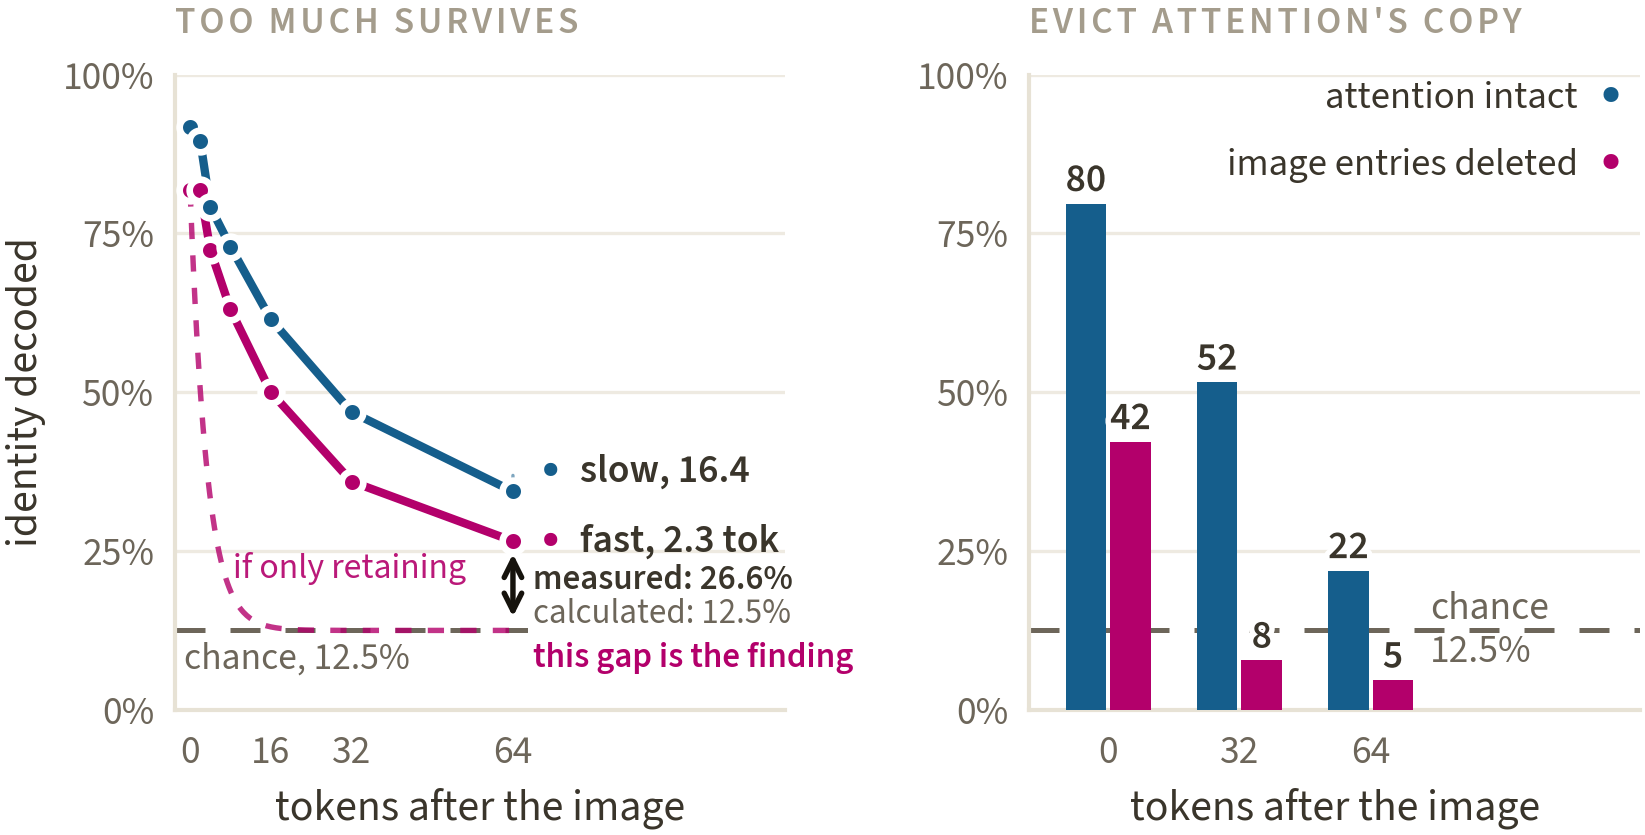
\includegraphics[width=\linewidth]{assets/f2_relay.png}
\caption{\textbf{Left: how to read this panel.} The two solid curves are
measurements: identity decoded from the slow and fast strata at matched write
gain, $n = 192$ per point. The dashed curve is not a measurement but a
calculation: where the fast stratum would read if its signal came only from
what its own $2.3$-token half-life retains. The calculation reaches chance
within ten tokens; the measurement ends at $26.6\%$ at $d{=}64$. The
slow-above-fast ordering is what decay predicts; the gap between the two fast
curves is what decay cannot explain.
\textbf{Right:} the same recurrent state probed with and without the attention
channel's copy of the image, fast tercile, $n = 64$ per bar. The eviction
happens immediately after the image is read and never touches the recurrent
state, which is identical in both runs at that instant.}
\label{fig:relay}
\end{figure}

But now look at the amounts, because they are the finding. A stratum with a
predicted half-life of $2.3$ tokens retains
$2^{-64/2.3} \approx 4\times10^{-9}$ of anything it wrote sixty-four tokens
ago. Yet it reads $26.6\%$ there, twice the chance rate
($p = 1\times10^{-7}$, $n = 192$), and the measured half-life of its readout
is $19.3$ tokens, eight times its prediction. The slow stratum overshoots in
the same direction: predicted $16.4$ tokens, measured $26.3$, with four times
more signal surviving at $d{=}64$ than its parameters allow. In short, the
strata are ordered exactly as decay predicts, and both hold far more signal
than decay permits.

One caveat applies to any global split of this kind. The strata draw unequal
numbers of heads from each layer, and depth matters a great deal for decoding,
so the comparison between strata carries a depth component. The comparison of
each stratum with its own prediction does not: whatever layers the fast
stratum draws from, its own decay parameters bound what it can retain, and it
reads far above that bound.

\keyfinding{With write amplitude held fixed, the strata are ordered exactly as
decay predicts, and both hold far more signal than decay permits. A head with
a two-token half-life cannot be holding something written sixty-four tokens
earlier: by then its state consists almost entirely of recent writes. If such
heads still decode object identity at twice chance, the identity information
in their state arrived recently. Something else in the model must be supplying
it.}

\section{Result 3: The Recurrent Channel Is a Relay, Not a Store}
\label{sec:relay}

What could be supplying it? Only one component of the model still holds the
image at distance: the attention channel, whose key-value entries do not
decay. We tested this directly. Each trial was run twice, identically, except
that in one run we deleted the image's key-value entries from all 13 attention
layers immediately after the image was read, \emph{before a single filler
token was processed}. The deletion does not touch the recurrent state. At that
instant, the recurrent state is identical in both runs.

The two hypotheses now make opposite predictions. If the recurrent state is
remembering the image on its own, deleting attention's copy should not change
what a probe reads from the state. If the state is being refreshed from
attention, the deletion should collapse decodability at distance, and it
should hurt the fast heads most, because they depend most on being refreshed.

\begin{table}[h]
\centering\small
\begin{tabular}{lrrrr}
\toprule
stratum & distance & visual KV intact & visual KV evicted & change \\
\midrule
fast   & 0  & $79.7\%$ & $42.2\%$ & $-37.5$ \\
fast   & 32 & $51.6\%$ & $\mathbf{7.8\%}$  & $-43.7$ \\
fast   & 64 & $21.9\%$ & $4.7\%$  & $-17.2$ \\
\addlinespace
middle & 0  & $62.5\%$ & $43.8\%$ & $-18.8$ \\
slow   & 0  & $62.5\%$ & $54.7\%$ & $-7.8$  \\
\addlinespace
all    & 0  & $59.4\%$ & $59.4\%$ & $0.0$   \\
all    & 32 & $6.2\%$  & $6.2\%$  & $0.0$   \\
\bottomrule
\end{tabular}
\caption{Identity decodability from the recurrent state with and without the
attention channel's copy of the image, $n = 64$ per cell. Chance is $12.5\%$.
The fast heads' apparent memory at 32 tokens is entirely dependent on the
attention channel: removing it drops them from $51.6\%$ to below chance.}
\label{tab:relay}
\end{table}

\begin{figure}[h]
\centering

\includegraphics[width=\linewidth]{assets/f3_controls.png}
\caption{\textbf{Left: read this panel vertically.} At every x position,
compare each curve with the no-eviction baseline: the text-eviction curve
sits above it everywhere, the image-eviction curve below it. Both deletions
remove the same number of positions from the same 13 caches, so damage alone
cannot explain opposite signs. \textbf{Right:} accuracy lost when the visual
entries are zeroed at all 13 attention layers, at only the earliest three,
and at only the latest three. The earliest three reproduce most of the full
effect; the latest three do nothing, so visual information enters early.}
\label{fig:controls}
\end{figure}

There is a fair objection to the eviction experiment: deleting entries
shortens every cache and changes the softmax normalisation, so perhaps we
damaged the machinery rather than removed a memory. The control is to delete
the same \emph{number} of positions from the same caches, but delete text
instead of the image. The two versions do identical mechanical damage, so if
damage were the explanation, both should push the reading down. Instead they
move it in opposite directions (Figure~\ref{fig:controls}, left): at 32
tokens, deleting the image costs the fastest decile $18.8$ points while
deleting an equal number of pre-image text positions \emph{raises} it by
$29.7$; averaged over ten deciles the effects are $-6.4$ and $+12.5$ points.
Damage cannot push a reading up.

\subsection{The decay parameters predict how much is relayed}

Result 2 found that the parameter-derived horizon does not predict the
measured decodability curve. It does predict something else, and that
something is exactly what the relay account says it should predict. Reason it
through: a head that forgets quickly must depend more heavily on being
refreshed, so deleting the source of the refresh should hurt its readout more.
Ordering the strata by decay rate shows exactly this pattern. The size of the
effect depends on how the strata are formed:

\begin{table}[h]
\centering\small
\begin{tabular}{llrrr}
\toprule
split & stratum & predicted $t_{1/2}$ & intact at $d{=}0$ & drop under eviction \\
\midrule
tercile      & fast & $1.98$  & $79.7\%$ & $37.5$ points \\
tercile      & slow & $28.96$ & $62.5\%$ & $7.8$ points \\
\addlinespace
gain-matched & fast & $2.30$  & $52.6\%$ & $22.4$ points \\
gain-matched & slow & $16.35$ & $69.8\%$ & $9.4$ points \\
\bottomrule
\end{tabular}
\caption{Dependence on the attention channel at $d{=}0$, against the decay
rate implied by each stratum's own $A$ and gate. Terciles: $n = 64$ per cell;
gain-matched: $n = 192$ per cell. The tercile contrast reaches $4.8\times$ but
confounds decay with write amplitude; at matched amplitude the ratio is
$2.4\times$. The two splits come from different collections, so accuracies are
comparable within a split, not across splits.}
\label{tab:dose}
\end{table}

Note that each row of this table compares intact against evicted \emph{on the
same heads}, so write amplitude cancels within a row. The amplitude confound
affects only comparisons between strata. This is why the ratio worth quoting
is the gain-matched one. At thirty-two tokens the gain-matched fast stratum
reads only five points above chance even when intact, so eviction has little
left to remove, and the contrast is uninformative there. The decay calculation
therefore does carry predictive content, but about the mechanism rather than
about the decay curve: it identifies which heads are relaying and which are
retaining. The effect is half the size the confounded split suggested, and it
is measured at one distance on two strata. We flag both points in the
limitations.

The headline contrast is large. At 32 tokens, the fast tercile reads $51.6\%$
with the attention channel intact and $7.8\%$ without it, which is below the
$12.5\%$ chance rate. In raw counts, thirty-three correct predictions out of
sixty-four become five. Meanwhile the slow heads at distance zero, whose
content was written while the image was still being read, are barely affected
by eviction ($62.5\%$ to $54.7\%$). This is the control showing that the
intervention does not simply break the model.

\keyfinding{What a probe reads out of the recurrent state at distance is not
what the state remembered. It is what the attention channel is still supplying,
continuously re-supplied while that copy is present. Our evidence does not
distinguish re-encoding at every token from a single re-supply shortly after the
image, so we claim the dependence, not its period. The recurrent channel relays
the picture; it does not store it.}

\subsection{What the probe can see, and why that matters here}

There is one more objection to consider: perhaps the probe is simply
insensitive to weak signals. Freshly re-encoded content plausibly sits at
higher amplitude than content written long ago and decayed. A probe that finds
strong signals and misses faint ones could then produce all of our
observations even if the state never stopped storing the image.

This objection can be measured, and we measured it. We take the distance-zero
features, where the image is present at full strength, and artificially weaken
each trial's own contribution while substituting an equal amount of unrelated
variation from another trial, keeping total variance roughly constant:
$x_i(\alpha) = \mu + \alpha (x_i - \mu) + \sqrt{1-\alpha^2}\,(x_j - \mu)$.
This transformation mimics what decay followed by overwriting does to a stored
trace: the signal shrinks while unrelated content takes its place.

The result gives the probe a detection floor. The probe loses half its signal
at $\alpha = 0.78$ and cannot be distinguished from chance by
$\alpha \approx 0.25$. The best single-layer probe behaves the same way,
halving at $\alpha = 0.75$. In plain terms, this instrument cannot see content
below roughly a quarter of full amplitude.

Now put that floor next to the prediction. The weights say that after
thirty-two tokens, a retained trace sits at $3.7\%$ of full amplitude at the
median head and $18\%$ at the mean, both below the floor. So a genuinely
retained trace at that distance \emph{could not} produce a visible reading.
Yet the intact probe reads the fast heads at $51.6\%$ there. Whatever the
probe is reading must therefore be high in amplitude, which means recently
written. And deleting the attention channel's copy removes it.

\begin{figure}[h]
\centering
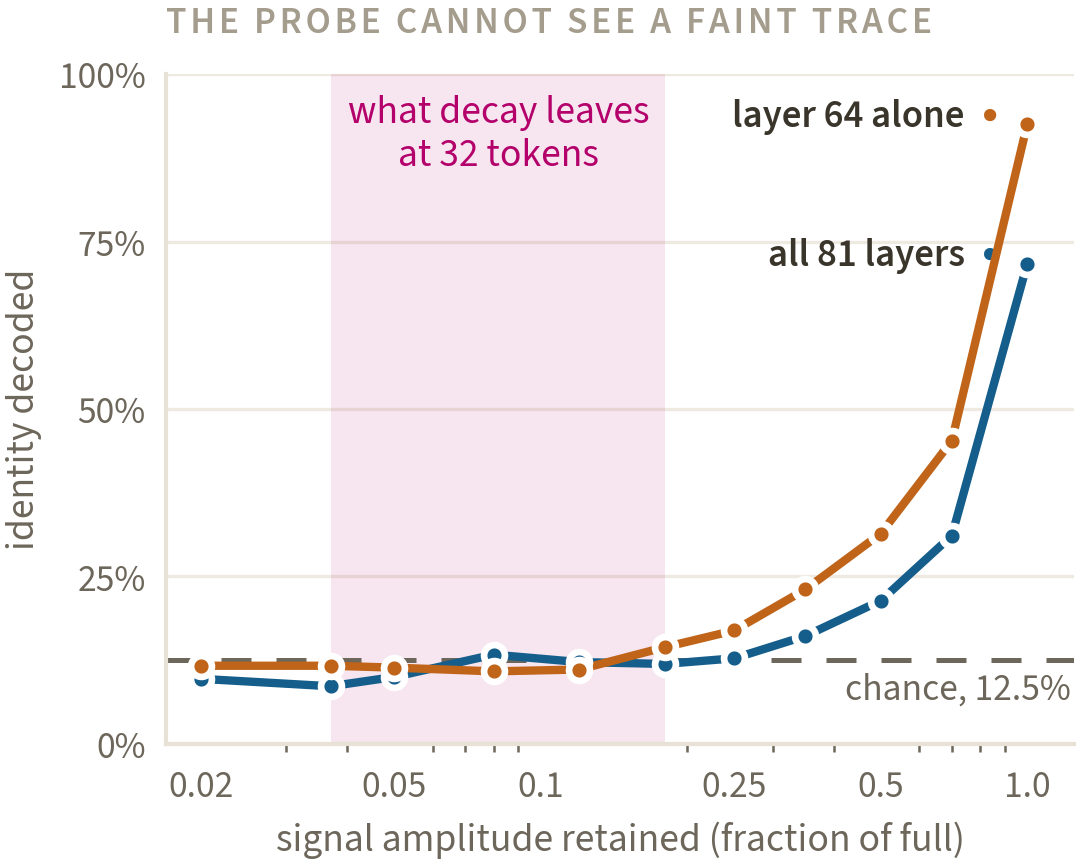
\includegraphics[width=0.72\linewidth]{assets/f4_sensitivity.png}
\caption{How faint a signal the probe can still recover. Each trial's own
contribution is attenuated while an equal amount of unrelated variation is
substituted, holding total variance roughly constant. The shaded band is what
the model's decay parameters leave of a stored trace after 32 tokens, between
the median and the mean over heads. Both probes are at chance throughout that
band, so a visible reading at 32 tokens cannot be a retained one.}
\label{fig:sensitivity}
\end{figure}

\keyfinding{The probe's insensitivity to faint signals is what makes the
positive reading informative. A signal the instrument can see at thirty-two
tokens is necessarily a fresh one, because a retained one would be four to six
times below its detection floor.}

The same measurement bounds what we may conclude. Whether faint retained content
persists below the floor is not answerable with this instrument at any distance
beyond a few tokens, so this paper does not claim the state stops storing the
image. It claims that what a probe reads at distance is not retention, and that
it depends causally on the attention channel.

This one measurement explains three earlier puzzles. First, it explains why
the measured horizon exceeds the predicted one, and why the gap grows in
smaller models: the probe was never measuring retention in the first place.
Second, it explains why the tercile split made the fast heads look like the
best retainers: they write hardest, so whatever the attention channel
re-supplies lands in them at the highest amplitude, and holding the write gain
fixed removes that apparent advantage (Section~\ref{sec:strata}). Third, it
supplies the mechanism behind the causal result, which the next section takes
up.

\section{Result 4: Causally, the Answer Follows the Attention Channel}

The probe results say the attention channel supplies what the recurrent state
appears to hold. The splice tests the same claim on the model's own behaviour,
with no probe involved. Recall the setup: two runs see different images, one
memory channel is exchanged between them, and the host run then answers its
question. We admit a pair only if the host and the donor each answered their
own question correctly beforehand, so the ceiling is $100\%$ by construction.
Of 111 attempted pairs, 11 were rejected on that criterion, and none were
rejected for mismatched cache length. Every recurrent swap was verified to
have changed the state, 100 of 100.

\begin{table}[h]
\centering\small
\begin{tabular}{lrrr}
\toprule
condition & layers swapped & follows host & follows donor \\
\midrule
no swap                       & 0  & $100/100$ $[96,100]$ & $0/100$ $[0,4]$ \\
recurrent, all 81 states      & 0  & $100/100$ $[96,100]$ & $0/100$ $[0,4]$ \\
\addlinespace
attention, 1 layer            & 1  & $100/100$ $[96,100]$ & $0/100$ $[0,4]$ \\
attention, 3 layers spread    & 3  & $98/100$ $[93,99]$   & $0/100$ $[0,4]$ \\
attention, 7 layers           & 7  & $4/100$ $[2,10]$     & $94/100$ $[88,97]$ \\
attention, all 13             & 13 & $0/100$ $[0,4]$      & $98/100$ $[93,99]$ \\
\addlinespace
attention, earliest 3         & 3  & $94/100$ $[88,97]$   & $1/100$ $[0,5]$ \\
attention, latest 3           & 3  & $100/100$ $[96,100]$ & $0/100$ $[0,4]$ \\
both channels                 & 13 & $0/100$ $[0,4]$      & $100/100$ $[96,100]$ \\
\bottomrule
\end{tabular}
\caption{The splice at 100 pairs with a $100\%$ ceiling. Brackets are $95\%$
Wilson intervals in percent. Replacing the entire recurrent memory of all 81
layers changes nothing; replacing seven of the thirteen attention caches flips
the answer to the other image.}
\label{tab:splice}
\end{table}

\begin{figure}[h]
\centering
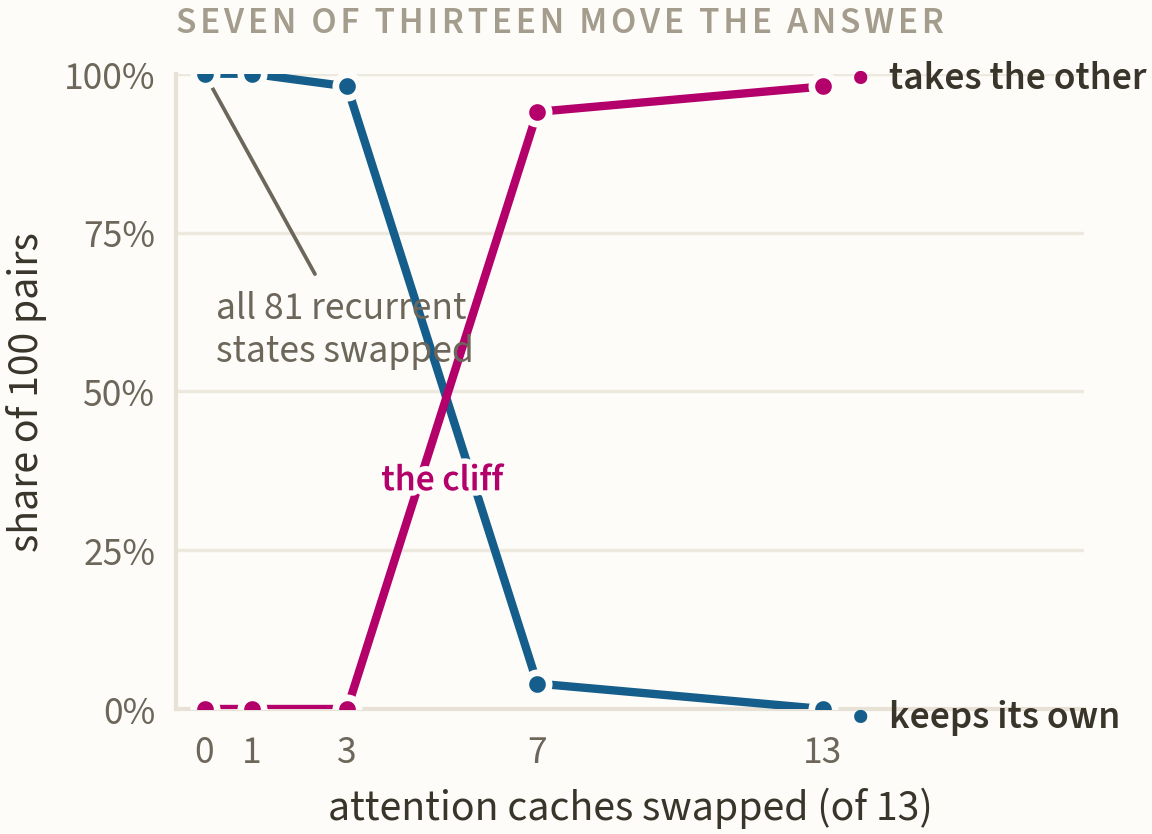
\includegraphics[width=0.72\linewidth]{assets/f5_splice.png}
\caption{How many of the thirteen attention caches must be exchanged before the
answer follows the other image, over 100 pairs in which both images were
answered correctly beforehand. The leftmost point is the recurrent swap: all 81
states replaced, no attention cache touched, no effect.}
\label{fig:splice}
\end{figure}

Three things can be read from Table~\ref{tab:splice} and
Figure~\ref{fig:splice}. First, replacing the recurrent memory has no effect
at all: exchanging all 81 recurrent states and convolution buffers leaves
$100$ of $100$ answers following the host's own image, with every swap
verified to have taken effect. Second, the attention channel is causally
sufficient to determine the answer: swapping seven of the thirteen caches
moves $94$ of $100$ answers to the donor's image. Third, the dependence on
attention is graded and distributed. One swapped attention layer changes
nothing, three spread across the stack move two answers, and seven move almost
all of them. No small subset of layers is enough, so the picture is held
across the attention layers rather than concentrated in a few. The earliest
three layers have a small effect and the latest three have none, which matches
visual information entering early and being consumed downstream.

Why does replacing the entire recurrent memory change nothing? Result 3
already answers this. The transplanted state is decayed away within a few
tokens and rewritten from the attention channel, which the recurrent swap
leaves untouched. The probe result and the splice result are the same fact
seen from two sides.

\keyfinding{In the earlier version of this work, the same splice gave a host
baseline of 17 of 30. That figure was an artefact of our own instrument: the
question was fed through the cache without the generation prompt the model
expects, so the model often continued the prompt instead of answering.
Correcting the prompt format lifts the baseline to $100\%$ and leaves the
direction of every conclusion unchanged.}

\section{Result 5: Scale, and Where the Prediction Fails}

We repeated the core protocol at three model scales. The instruments read
every tensor shape from the loaded model's configuration rather than assuming
the 7B geometry. This is a requirement, not a convenience: the 2.7B and 1.2B
checkpoints use a single B/C group where the 7B uses two, and the 1.2B has a
state dimension of 128 where the others have 64. Table~\ref{tab:scale}
reports the results.

\begin{table}[h]
\centering\small
\begin{tabular}{lrrrrrr}
\toprule
model & layers & attn & probe $d{=}0$ & probe $d{=}64$ & measured $t_{1/2}$ & predicted $t_{1/2}$ \\
\midrule
Zamba2-VL-7B   & 81 & 13 & $71.7\%$ & $21.7\%$ & $4.0$  & $6.64$ \\
Zamba2-VL-2.7B & 54 &  9 & $84.2\%$ & $31.7\%$ & $9.6$  & $2.91$ \\
Zamba2-VL-1.2B & 38 &  6 & $83.3\%$ & $34.2\%$ & $14.3$ & $2.58$ \\
\bottomrule
\end{tabular}
\caption{The same protocol at three scales, 120 identity trials per distance.
The pre-image control reads exactly $12.5\%$ at every scale. Half-lives are in
tokens: measured is the distance at which above-chance decodability halves,
predicted is the median over heads of $\ln 2/(|A|\bar{\Delta})$.}
\label{tab:scale}
\end{table}

Two conclusions follow. The second is a negative result, and we report it
plainly.

First, the parameter-derived horizon is short at every scale. Median predicted
half-lives are $6.64$, $2.91$ and $2.58$ tokens, and the fraction of heads
with a predicted half-life under 32 tokens is $85.0\%$, $97.9\%$ and $95.6\%$.
Whatever the recurrent state genuinely retains of its own past, it retains it
for single-digit token counts in all three models.

Second, the predicted horizon does not predict the measured one. Across the
three models the two quantities move in opposite directions: the prediction
falls with scale while the measurement rises. On the 7B alone the agreement
looked strong, with measured decodability tracking predicted retention at
$r = 0.973$ across eleven distances. That agreement does not replicate at the
other scales. We therefore do not claim that the decay calculation explains
the measured decay curve. Result 3 already showed why it cannot: the probe at
distance is reading relayed content, not retained content, so its curve is not
governed by the decay parameters.

\section{Result 6: Visual Key-Value Eviction Removes the Only Copy, Eventually}

Pruning methods discard visual key-value entries on the premise that they are
redundant. Our results say the redundancy comes from the relay, and the relay
is short-lived, so the premise should degrade with distance. We test this
directly on the model's own behaviour. We evict a fraction of the visual
key-value entries from all 13 attention layers immediately after the image is
read, let the filler and the question stream past the pruned cache, and
measure the model's accuracy. Retention $\rho$ is the fraction of visual
positions kept, sampled uniformly, and the question is asked $d$ tokens after
the image.

\begin{table}[h]
\centering\small
\begin{tabular}{lrrrr}
\toprule
visual KV retained & $d{=}0$ & $d{=}32$ & $d{=}128$ & $d{=}512$ \\
\midrule
$100\%$ & $97.9\%$ & $95.8\%$ & $100.0\%$ & $97.9\%$ \\
$25\%$  & $91.7\%$ & $95.8\%$ & $95.8\%$  & $91.7\%$ \\
$5\%$   & $87.5\%$ & $77.1\%$ & $75.0\%$  & $64.6\%$ \\
$0\%$   & $64.6\%$ & $37.5\%$ & $31.2\%$  & $22.9\%$ \\
\bottomrule
\end{tabular}
\caption{Behavioural accuracy under visual key-value eviction, against distance
between the image and the question. $n = 48$ per cell, chance $12.5\%$, no
failures. The unpruned row is flat, so distance alone costs nothing.}
\label{tab:eviction}
\end{table}

Table~\ref{tab:eviction_cost} reads the same data as cost, relative to the
unpruned baseline at the same distance:

\begin{table}[h]
\centering\small
\begin{tabular}{lrrrr}
\toprule
visual KV retained & $d{=}0$ & $d{=}32$ & $d{=}128$ & $d{=}512$ \\
\midrule
$25\%$ & $6.2$  & $0.0$  & $4.2$  & $6.2$ \\
$5\%$  & $10.4$ & $18.8$ & $25.0$ & $33.3$ \\
$0\%$  & $33.3$ & $58.3$ & $68.8$ & $75.0$ \\
\bottomrule
\end{tabular}
\caption{Accuracy points lost to pruning, relative to the unpruned baseline at
the same distance.}
\label{tab:eviction_cost}
\end{table}

With a quarter of the entries retained, there is no distance effect at all:
the cost is $6.2$, $0.0$, $4.2$ and $6.2$ points, flat within noise. At that
level the redundancy premise holds on this architecture, and we found no
evidence against it.

Below that level, distance starts to matter, and it matters a great deal. At a
twentieth retained, the cost triples across the range, from $10.4$ points
beside the image to $33.3$ points at 512 tokens. With every visual entry
removed, it runs from $33.3$ to $75.0$. Compare the unpruned row, which is
flat across the same distances. So the problem is not that long prompts are
hard. The problem is that long prompts become hard \emph{once the visual
entries are gone}, because by then the recurrent channel has nothing left to
relay from.

\begin{figure}[h]
\centering

\includegraphics[width=0.72\linewidth]{assets/f6_eviction.png}
\caption{Model accuracy under visual key-value eviction, against how far the
question sits from the image, $n = 48$ per point. The unpruned line is flat, so
distance alone costs nothing. Keeping a quarter of the entries is also flat.
Below that the lines fan out: the cost of pruning grows with distance only once
the recurrent channel has stopped relaying the picture.}
\label{fig:eviction}
\end{figure}

\keyfinding{The cost of heavy pruning is not one number. Above a retention
threshold, somewhere between a quarter and a twentieth on this model, pruning
costs the same at every distance. Below it, the cost grows with how far the
question sits from the image: a method validated at short range will
understate its cost at long range by a factor of three at $5\%$ retention.}

The zero-retention row also gives the cleanest available measure of what the
recurrent channel contributes on its own. With no visual entries anywhere in
the attention caches, the model can only be answering from its recurrent
states. Its accuracy falls from $64.6\%$ beside the image to $22.9\%$ at 512
tokens. That decline is the recurrent channel's own contribution decaying,
measured on behaviour with an instrument entirely independent of the probe,
and it agrees with the picture the probe gives.

One discrepancy should be stated plainly. At zero retention the model still
answers at $37.5\%$ at thirty-two tokens, well above the $12.5\%$ chance rate,
while our linear probe reads the recurrent state at close to chance at that
distance. So the model is using something in the recurrent channel that the
probe does not recover. The probe is a lower bound on what the state carries,
not a full measure of it. The sentence ``the state is empty'' is not supported
by our evidence, and we do not claim it.

\section{Limitations}

We separate three kinds of limitation: alternative explanations our evidence
does not exclude, limits on what the instruments can see, and limits on scope.
The first kind is the one that should decide how much weight a reader puts on
the central claim, so it comes first.

\subsection{Alternative explanations we have not excluded}

\textbf{Eviction changes more than the image's presence, though the matched
control argues against this.} Removing the visual key-value entries shortens
every attention layer's cache by roughly 400 positions and changes the
softmax normalisation for every token that follows. The matched control
(Section~\ref{sec:relay}) deletes an equal number of \emph{non-visual}
positions from the same caches, and the two deletions move the readout in
opposite directions, which pure damage cannot produce. A narrower version of
the worry survives: the pre-image text we remove does not contribute to the
residual stream the way the image does, so the comparison bounds the damage
account rather than eliminating every version of it.

\textbf{The relay result could be a sensitivity asymmetry.} Our own data show
the probe is a lower bound (below), and a lower bound need not be a uniform
one. Freshly re-encoded content plausibly sits at higher amplitude in the state
than content written many tokens earlier and decayed. If the probe recovers
high-amplitude content easily and low-amplitude content poorly, then removing
the re-encoded copy would collapse the readout even in a state that was still
genuinely retaining something. That account predicts the same observations we
report. Distinguishing it requires either a probe whose sensitivity is
calibrated against signal amplitude, or a model with no attention channel to
relay from, where probing the recurrent state must be measuring retention
because there is nothing else it could be measuring.

\textbf{The route is not traced.} The eviction contrast shows that decodable
identity at distance depends on the attention channel holding the image. It
does not show the path. The natural account is that attention layers write
image-derived content into the residual stream and downstream Mamba2 mixers
re-encode it, but a layerwise eviction, removing the visual entries from only
the early or only the late attention layers, would be needed to establish it and
we have not run one.

\subsection{What the instruments can and cannot see}

\textbf{The probe is a lower bound, and our own behavioural data prove it.}
With every visual key-value entry removed, the model answers at $37.5\%$ at
thirty-two tokens while the probe reads the recurrent state near chance at the
same distance. Something usable survives there that a 512-dimensional random
projection, read by a linear probe trained on 120 examples, does not recover.
Every statement in this paper about what the state contains should be read as a
statement about what is linearly decodable under that instrument. The paper does
not establish that the state is empty of the image at any distance, and readers
should not take the phrase ``the state empties'' from the earlier version of
this work as supported.

\textbf{Probe accuracy depends on the feature-to-trial ratio.} Count read at
chance with 128 projection features and reached $19.4\%$ at 512. In the other
direction, the full $41{,}472$-dimensional state probe reads $71.7\%$ where a
single layer's 512 features read $92.5\%$ on identical trials. Absolute
accuracies are therefore not comparable across collections of different size or
width, and we report them only within a collection. The decay curve in
Table~\ref{tab:fine} is internally consistent because the same 120 trials appear
at every distance.

\textbf{One projection basis, one seed.} Every probe result uses a single fixed
Gaussian projection. We have not repeated the analysis across projection seeds,
so the variance attributable to the choice of basis is unmeasured.

\textbf{The stratum dose-response is confirmed at matched amplitude only at
distance zero.} On the tercile split eviction sensitivity is ordered exactly
by predicted decay rate ($37.5$, $18.8$ and $7.8$ points, $r = 0.991$), but
every split by half-life is also a split by write amplitude. With the gate
held fixed the ratio is $2.4\times$ at distance zero over two strata at
$n = 192$, and unmeasurable at thirty-two tokens, where the gain-matched fast
stratum reads too close to chance intact for eviction to have anything to
remove. Two strata at one distance in one model is a direction, not a curve.

\subsection{Scope}

\textbf{One model family, and a second family we tried and failed on.} Results
come from three Zamba2-VL checkpoints, which is one vendor, one architecture
family and one training recipe. This is the principal limit on the paper's
generality and we do not argue around it.

We attempted to extend the relay result to a second family and report the
attempt because its failure is informative. Granite 4.0 h-tiny \cite{granite4} is a Mamba2
hybrid from a different lineage, with 36 recurrent layers to 4 attention layers
against Zamba2-VL-7B's 81 to 13. Its decay parameters read out cleanly and give
a median predicted half-life of $8.7$ tokens, so the horizon calculation of
Section 5 transfers to a second family. The relay contrast does not, for an
instrumental reason: on a code-word recall task the model answers correctly on
$100\%$, $96.9\%$ and $100\%$ of trials at $0$, $32$ and $64$ tokens, and yet a
probe on its recurrent state reads at chance at distance zero. Scaling to 256
trials did not change this ($13.7\%$ against a $12.5\%$ chance rate,
$p = 0.31$), and neither did probing single layers, where the best of 36 layers
reached $19.9\%$.

We suspected the item was too small to write a detectable trace, a one-token
code word against a 345-token image, and tested that by repeating the carrier
sixteen times so the item occupied 192 tokens. It did not help: $12.0\%$,
$17.2\%$ and $10.9\%$ across the three strata. Repetition lengthens an item
without diversifying what it writes, so the state ends up holding little more
than the final repeat, which is not the manipulation we intended. We do not
know why the instrument fails on this model; we only know that it does. No
relay claim can be made beyond the Zamba2-VL family on this evidence. A
vision-language hybrid from a second family, where the item
is a real image, remains the right test and we have not run it. The sharper
version of that test is a vision-language model with no attention layers at all,
such as Cobra \cite{zhao2025cobra} or VL-Mamba \cite{qiao2024vlmamba}, where
probing the recurrent state must be measuring retention because there is nothing
else it could be measuring. Both are Mamba1 models and would need the read
operator ported before any number from them could be trusted.

\textbf{One task format, one dataset, one modality.} Eight-way forced choice on
COCO buys an exact chance rate and a clean pre-image control, and costs
generality to free-form answering, to other visual properties, and to whether
any of this holds for text held in the same states.

\textbf{The horizon is measured on one filler distribution.} $\bar{\Delta}$ is
input dependent. We measured it on natural prose and found the median half-life
stable across images, from $6.44$ to $6.86$ tokens, but a filler with very
different gate statistics would give a different horizon, which the same
calculation would predict.

\textbf{An instrument artefact we corrected, and what it implies.} The splice
reported in the earlier version of this work fed the question through the cache
without the generation prompt the model expects. The model frequently continued
the prompt rather than answering it, naming every candidate and scoring as
ambiguous, which is why the host baseline read 17 of 30. Under the corrected
format the baseline is $100/100$. The direction of every conclusion is
unchanged, but the earlier absolute rates were a property of our instrument
rather than of the model. We report both so the difference is auditable, and we
note the general lesson: a null result measured through a degraded instrument is
worth less than its sample size suggests.

\section{Conclusion}

The recurrent state of this hybrid vision-language model is not a memory of
the image in any useful sense. It is a selective summary of the picture's
gist, and it holds that summary for only about four tokens. That lifetime is
not an empirical curiosity: it can be computed from the model's own decay
parameters before any measurement is taken. What the model actually answers
from lives in the thin attention channel, and the recurrent state relays that
content rather than storing its own copy. The practical consequence is direct:
the visual key-value entries a hybrid carries are redundant only for as long
as the recurrent state is still relaying the picture, and that is not long.

\begin{thebibliography}{99}\small\setlength{\itemsep}{1pt}

\bibitem{katharopoulos2020linear}
A.~Katharopoulos, A.~Vyas, N.~Pappas, and F.~Fleuret.
\newblock Transformers are RNNs: Fast Autoregressive Transformers with Linear
Attention. \emph{ICML}, 2020.

\bibitem{gu2022s4}
A.~Gu, K.~Goel, and C.~R\'e.
\newblock Efficiently Modeling Long Sequences with Structured State Spaces.
\emph{ICLR}, 2022.

\bibitem{peng2023rwkv}
B.~Peng, E.~Alcaide, Q.~Anthony, A.~Albalak, S.~Arcadinho, S.~Biderman, et~al.
\newblock RWKV: Reinventing RNNs for the Transformer Era.
\emph{arXiv:2305.13048}, 2023.

\bibitem{gu2023mamba}
A.~Gu and T.~Dao.
\newblock Mamba: Linear-Time Sequence Modeling with Selective State Spaces.
\emph{arXiv:2312.00752}, 2023.

\bibitem{dao2024mamba2}
T.~Dao and A.~Gu.
\newblock Transformers are SSMs: Generalized Models and Efficient Algorithms
Through Structured State Space Duality. \emph{ICML}, 2024.

\bibitem{beck2024xlstm}
M.~Beck, K.~P\"oppel, M.~Spanring, A.~Auer, O.~Prudnikova, M.~Kopp,
G.~Klambauer, J.~Brandstetter, and S.~Hochreiter.
\newblock xLSTM: Extended Long Short-Term Memory.
\emph{arXiv:2405.04517}, 2024.

\bibitem{lieber2024jamba}
O.~Lieber, B.~Lenz, H.~Bata, G.~Cohen, J.~Osin, I.~Dalmedigos, et~al.
\newblock Jamba: A Hybrid Transformer-Mamba Language Model.
\emph{arXiv:2403.19887}, 2024.

\bibitem{glorioso2024zamba}
P.~Glorioso, Q.~Anthony, Y.~Tokpanov, J.~Whittington, J.~Pilault, A.~Ibrahim,
and B.~Millidge.
\newblock Zamba: A Compact 7B SSM Hybrid Model.
\emph{arXiv:2405.16712}, 2024.

\bibitem{de2024griffin}
S.~De, S.~L. Smith, A.~Fernando, A.~Botev, G.~Cristian-Muraru, A.~Gu, et~al.
\newblock Griffin: Mixing Gated Linear Recurrences with Local Attention for
Efficient Language Models. \emph{arXiv:2402.19427}, 2024.

\bibitem{ren2025samba}
L.~Ren, Y.~Liu, Y.~Lu, Y.~Shen, C.~Liang, and W.~Chen.
\newblock Samba: Simple Hybrid State Space Models for Efficient Unlimited
Context Language Modeling. \emph{ICLR}, 2025.

\bibitem{waleffe2024empirical}
R.~Waleffe, W.~Byeon, D.~Riach, B.~Norick, V.~Korthikanti, T.~Dao, A.~Gu,
et~al.
\newblock An Empirical Study of Mamba-based Language Models.
\emph{arXiv:2406.07887}, 2024.

\bibitem{jelassi2024copying}
S.~Jelassi, D.~Brandfonbrener, S.~M. Kakade, and E.~Malach.
\newblock Repeat After Me: Transformers are Better than State Space Models at
Copying. \emph{arXiv:2402.01032}, 2024.

\bibitem{merrill2024illusion}
W.~Merrill, J.~Petty, and A.~Sabharwal.
\newblock The Illusion of State in State-Space Models. \emph{ICML}, 2024.

\bibitem{wen2024rnns}
K.~Wen, X.~Dang, and K.~Lyu.
\newblock RNNs are not Transformers (Yet): The Key Bottleneck on In-context
Retrieval. \emph{arXiv:2402.18510}, 2024.

\bibitem{arora2023zoology}
S.~Arora, S.~Eyuboglu, A.~Timalsina, I.~Johnson, M.~Poli, J.~Zou, A.~Rudra,
and C.~R\'e.
\newblock Zoology: Measuring and Improving Recall in Efficient Language Models.
\emph{arXiv:2312.04927}, 2023.

\bibitem{arora2024based}
S.~Arora, S.~Eyuboglu, M.~Zhang, A.~Timalsina, S.~Alberti, D.~Zinsley, J.~Zou,
A.~Rudra, and C.~R\'e.
\newblock Simple Linear Attention Language Models Balance the Recall-Throughput
Tradeoff. \emph{arXiv:2402.18668}, 2024.

\bibitem{alain2016probes}
G.~Alain and Y.~Bengio.
\newblock Understanding Intermediate Layers Using Linear Classifier Probes.
\emph{arXiv:1610.01644}, 2016.

\bibitem{hewitt2019control}
J.~Hewitt and P.~Liang.
\newblock Designing and Interpreting Probes with Control Tasks.
\emph{EMNLP}, 2019.

\bibitem{belinkov2022probing}
Y.~Belinkov.
\newblock Probing Classifiers: Promises, Shortcomings, and Advances.
\emph{Computational Linguistics}, 2022.

\bibitem{vig2020causal}
J.~Vig, S.~Gehrmann, Y.~Belinkov, S.~Qian, D.~Nevo, S.~Sakenis, J.~Huang,
Y.~Singer, and S.~Shieber.
\newblock Causal Mediation Analysis for Interpreting Neural NLP: The Case of
Gender Bias. \emph{arXiv:2004.12265}, 2020.

\bibitem{meng2022rome}
K.~Meng, D.~Bau, A.~Andonian, and Y.~Belinkov.
\newblock Locating and Editing Factual Associations in GPT.
\emph{NeurIPS}, 2022.

\bibitem{wang2022ioi}
K.~Wang, A.~Variengien, A.~Conmy, B.~Shlegeris, and J.~Steinhardt.
\newblock Interpretability in the Wild: a Circuit for Indirect Object
Identification in GPT-2 small. \emph{arXiv:2211.00593}, 2022.

\bibitem{zhang2024patching}
F.~Zhang and N.~Nanda.
\newblock Towards Best Practices of Activation Patching in Language Models:
Metrics and Methods. \emph{ICLR}, 2024.

\bibitem{chen2024fastv}
L.~Chen, H.~Zhao, T.~Liu, S.~Bai, J.~Lin, C.~Zhou, and B.~Chang.
\newblock An Image is Worth 1/2 Tokens After Layer 2: Plug-and-Play Inference
Acceleration for Large Vision-Language Models. \emph{ECCV}, 2024.

\bibitem{yang2024visionzip}
S.~Yang, Y.~Chen, Z.~Tian, C.~Wang, J.~Li, B.~Yu, and J.~Jia.
\newblock VisionZip: Longer is Better but Not Necessary in Vision Language
Models. \emph{arXiv:2412.04467}, 2024.

\bibitem{shang2025prumerge}
Y.~Shang, M.~Cai, B.~Xu, Y.~J. Lee, and Y.~Yan.
\newblock LLaVA-PruMerge: Adaptive Token Reduction for Efficient Large
Multimodal Models. \emph{ICCV}, 2025.

\bibitem{zhang2023h2o}
Z.~Zhang, Y.~Sheng, T.~Zhou, T.~Chen, L.~Zheng, R.~Cai, Z.~Song, Y.~Tian,
C.~R\'e, C.~Barrett, Z.~Wang, and B.~Chen.
\newblock H\textsubscript{2}O: Heavy-Hitter Oracle for Efficient Generative
Inference of Large Language Models. \emph{arXiv:2306.14048}, 2023.

\bibitem{li2024snapkv}
Y.~Li, Y.~Huang, B.~Yang, B.~Venkitesh, A.~Locatelli, H.~Ye, T.~Cai, P.~Lewis,
and D.~Chen.
\newblock SnapKV: LLM Knows What You are Looking for Before Generation.
\emph{arXiv:2404.14469}, 2024.

\bibitem{xiao2024streaming}
G.~Xiao, Y.~Tian, B.~Chen, S.~Han, and M.~Lewis.
\newblock Efficient Streaming Language Models with Attention Sinks.
\emph{ICLR}, 2024.

\bibitem{liu2023llava}
H.~Liu, C.~Li, Q.~Wu, and Y.~J. Lee.
\newblock Visual Instruction Tuning. \emph{NeurIPS}, 2023.

\bibitem{bai2025qwen25vl}
S.~Bai, K.~Chen, X.~Liu, J.~Wang, W.~Ge, S.~Song, et~al.
\newblock Qwen2.5-VL Technical Report. \emph{arXiv:2502.13923}, 2025.

\bibitem{zhao2025cobra}
H.~Zhao, M.~Zhang, W.~Zhao, P.~Ding, S.~Huang, and D.~Wang.
\newblock Cobra: Extending Mamba to Multi-Modal Large Language Model for
Efficient Inference. \emph{AAAI}, 2025.

\bibitem{qiao2024vlmamba}
Y.~Qiao, Z.~Yu, L.~Guo, S.~Chen, Z.~Zhao, M.~Sun, Q.~Wu, and J.~Liu.
\newblock VL-Mamba: Exploring State Space Models for Multimodal Learning.
\emph{arXiv:2403.13600}, 2024.

\bibitem{lin2014coco}
T.-Y. Lin, M.~Maire, S.~Belongie, L.~Bourdev, R.~Girshick, J.~Hays, P.~Perona,
D.~Ramanan, C.~L. Zitnick, and P.~Doll\'ar.
\newblock Microsoft COCO: Common Objects in Context.
\newblock \emph{ECCV}, 2014. arXiv:1405.0312.

\bibitem{zamba2vl}
Zyphra.
\newblock Zamba2-VL-7B model card.
\newblock \url{https://huggingface.co/Zyphra/Zamba2-VL-7B}, 2026. Apache-2.0.

\bibitem{granite4}
IBM Granite Team.
\newblock Granite 4.0 h-tiny model card.
\newblock \url{https://huggingface.co/ibm-granite/granite-4.0-h-tiny}, 2025.

\end{thebibliography}

\end{document}
